\documentclass{article}
    \title{\vspace{-50pt}\textbf{\underline{COP4620 Quiz 5 Work}}}
    \author{}
    \date{}
    \usepackage[T1]{fontenc}
    \usepackage{algorithm}
    \usepackage{algpseudocode}
	\usepackage{enumitem}
    \usepackage{makecell}
    \usepackage{multicol}
    \usepackage{pifont}
    \usepackage{soul}
    \usepackage{tikz}
    \usepackage{titlesec}
    \usepackage[tmargin=1in,lmargin=1in,rmargin=1in]{geometry}
    \usetikzlibrary{automata, decorations.markings, positioning, arrows, arrows.meta, babel, positioning,shapes}
    \tikzset{
        ->, % makes the edges directed
        >=stealth', % makes the arrow heads bold
        node distance=3cm, % minimum distance between two nodes. Change if necessary.
        every state/.style={thick, fill=gray!10}, % sets properties for each state node
        initial text=$ $, % sets the text that appears on the start arrow
        line/.style={-},
    }
    \tikzset{
      blue  box/.style={ fill=blue!20,  draw=blue, minimum width={2*#1ex}, minimum height={2em} }
      green box/.style={ fill=green!20, draw=blue, minimum width={2*#1ex}, minimum height={2em} }
      red   box/.style={ fill=red!20,   draw=red,  minimum width={2*#1ex}, minimum height={2em} }
      gray  box/.style={ fill=gray!20,  draw=gray, minimum width={2*#1ex}, minimum height={2em} }
  	}
    \tikzstyle{vertex}=[draw,fill=black!15,circle,minimum size=20pt,inner sep=0pt]
    
    \algdef{SE}{Begin}{End}{\textbf{begin}}{\textbf{end}}

    \newcommand{\cmark}{\ding{51}}%
    \newcommand{\xmark}{\ding{55}}%
    \newcommand{\textb}[1]{\textcolor{blue}{#1}}
    \newcommand{\textg}[1]{\textcolor{green}{#1}}
    \newcommand{\textr}[1]{\textcolor{red}{#1}}

    \setlist[description]{noitemsep, topsep=0pt, itemsep=-.1em}
    \setlist[enumerate]{noitemsep, topsep=0pt, itemsep=-.1em}

    \newlength\tindent
    \setlength{\tindent}{\parindent}
    \setlength{\parindent}{0pt}
    \renewcommand{\indent}{\hspace*{\tindent}}

    \renewcommand{\familydefault}{\sfdefault}        	 
    \renewcommand\theadfont{\bfseries\sffamily}

	\titleformat{\chapter}[display]
	{\bfseries\Large\itshape}
	{Chapter\ \thechapter}{0.5ex}{ }

	\titleformat{\section}
	{\normalfont\bfseries}
	{\thesection}{0.5em}{}

	\titleformat{\subsection}
	{\normalfont\bfseries}
	{\thesubsection}{0.5em}{}
	
    \titlespacing\section{0pt}{12pt plus 4pt minus 8pt}{0pt plus 2pt minus 8pt}
    \titlespacing\subsection{0pt}{12pt plus 4pt minus 4pt}{0pt plus 2pt minus 4pt}

\begin{document}

\maketitle
\vspace{-60pt}

%\renewcommand\thechapter{Q1}
%\chapter{Take Home Quiz 4}

\section*{Question 2}
IR code is shown on left.  The corresponding generated Assembly code is shown on right. \\
Why is this assembly code not efficient?
\vspace{-1em}
\begin{multicols}{3}
 \ \\ \ \\ \ \\
\textr{ADD A, B, C} \\
\textb{ADD C, A, E}
\vfill\columnbreak
 \ \\ \ \\ \ \\
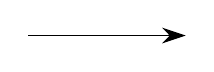
\begin{tikzpicture}
\draw [-{Stealth[length=3mm, width=2mm]}] (0,0) -- (2,0);
\end{tikzpicture}
\vfill\columnbreak
\textr{LD A, R1} \\
\textr{LD B, R2} \\
\textr{ADD R1, R2, R3} \\
\textr{ST R3, C} \\
\textb{LD C, R4} \\
\textb{LD A, R5} \\
\textb{ADD R4, R5, R6} \\
\textb{ST R6, E}
\end{multicols}
\begin{description}
  \item [\xmark] Redundant computation
  \item [\cmark] Redundant load of A \hspace{3.5em} (Loaded into R1 and R5)
  \item [\cmark] Use of too many registers \hspace{1.5em} (R4 and R5 are not necessary)
  \item [\cmark] Redundant load of C \hspace{3.5em} (C is already in R3, and loaded into R4) 
\end{description}


\section*{Question 3}
IR code is shown on left.  The corresponding generated Assembly code is shown on right. \\
Why is this assembly code not efficient?
\vspace{-1em}
\begin{multicols}{3}
 \ \\ \ \\ \ \\
\textr{ADD A, B, C} \\
\textb{ADD A, B, D}
\vfill\columnbreak
 \ \\ \ \\ \ \\
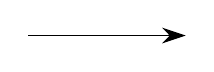
\begin{tikzpicture}
\draw [-{Stealth[length=3mm, width=2mm]}] (0,0) -- (2,0);
\end{tikzpicture}
\vfill\columnbreak
\textr{LD A, R1} \\
\textr{LD B, R2} \\
\textr{ADD R1, R2, R3} \\
\textr{ST R3, C} \\
\textb{LD A, R4} \\
\textb{LD B, R5} \\
\textb{ADD R4, R5, R6} \\
\textb{ST R6, D}
\end{multicols}
\begin{description}
  \item [\cmark] Redundant computation \hspace{2.1em} (Adding A and B twice, R1/R2, and R4/R5)
  \item [\cmark] Redundant load of A \hspace{3.5em} (Loaded into R1 and R4)
  \item [\xmark] Redundant load of C
  \item [\cmark] Redundant load of B \hspace{3.5em} (Loaded into R2 and R5) 
\end{description}


\section*{Question 4}
Perform Common Subexpression Elimination (CSE) on this code. Rather than generating assembly, just give new optimized 3AC. Use the exact same notation. Use exactly one space between symbols. \\
\begin{tabular}{|c|l|l|l}
  \hline
  \textbf{No.} & \textbf{3AC} & \textbf{Optimized 3AC} \\
  \hline
  1   & READ(A)     & READ(A) \\
  \hline
  2   & READ(B)     & READ(B) \\
  \hline
  3   & C = A + B   & C = A + B \\
  \hline
  4   & A = A + B   & A = C \\
  \hline
  5   & B = C * D   & \textbf{B = C * D} \\
  \hline
  6   & T1 = A + C  & \textbf{T1 = A + C} \\
  \hline
  7   & T2 = T1 + C & \textbf{T2 = T1 + C} \\
  \hline
  8   & F = A + C   & \textbf{F = T1} & \textr{$\leftarrow$ changed} \\
  \hline
  9   & C = F + B   & \textbf{C = F + B} \\
  \hline
  10  & G = A + C   & \textbf{G = A + C} \\
  \hline
  11  & T3 = F + B  & \textbf{T3 = C} & \textr{$\leftarrow$ changed} \\
  \hline
  12  & WRITE(T3)   & WRITE(T3) \\
  \hline
\end{tabular}


\newpage
\section*{Question 5}
Perform Common Subexpression Elimination (CSE) on this code. Rather than generating assembly, just give new optimized 3AC. Use the exact same notation. Use exactly one space between symbols.
\vspace{-1em}
\begin{multicols}{2}
\begin{tabular}{|c|l|l|l}
  \hline
  \textbf{No.} & \textbf{3AC} & \textbf{Optimized 3AC} \\
  \hline
  1   & A = 7       & A = 7 \\
  \hline
  2   & B = A + 2   & B = A + 2 \\
  \hline
  3   & C = A + B   & \textbf{C = A + B} \\
  \hline
  4   & D = C + B   & \textbf{D = C + B} \\
  \hline
  5   & A = D + C   & \textbf{A = D + C} \\
  \hline
  6   & B = D + C   & \textbf{B = A} & \textr{$\leftarrow$ changed} \\
  \hline
  7   & E = A + B   & \textbf{E = C} & \textr{$\leftarrow$ changed} \\
  \hline
  8   & F = D + C   & \textbf{F = A} & \textr{$\leftarrow$ changed} \\
  \hline
  9   & G = E + F   & \textbf{G = E + F} \\
  \hline
\end{tabular}
\begin{enumerate}
  \item How many expressions are available after processing line 8? \textbf{4} \\
  \item Which of the following expressions will be available after processing line 8?
  \begin{tabular}{|l|l|l|}
  \hline
  \textbf{No.} & \textbf{Expression} & \textbf{Available (y or n)} \\
  \hline
  1 & A+2 & n \\
  \hline
  2 & A+B & \textbf{y} \\
  \hline
  3 & C+B & \textbf{y} \\
  \hline
  4 & D+C & \textbf{y} \\
  \hline
  5 & E+F & \textbf{y} \\
  \hline
  \end{tabular}
\end{enumerate}
\end{multicols}


\section*{Question 6}
Perform \textit{liveness} analysis on this piece of code, assuming that it is the entire code of the program. Match the line number on the left-hand side with the \textit{live} sets on the right. \\
\begin{tabular}{|c|l|c|c|>{\bfseries}l|}
  \hline
  \textbf{No.} &  & \textbf{Defined} & \textbf{Used} & \textbf{Live} \\
  \hline
  1   & READ(A)     & -- & A     & \{A, B\} \\
  \hline
  2   & READ(B)     & -- & B     & \{A, B\} \\
  \hline
  3   & C = A + B   & C  & A, B  & \{A, B, C\} \\
  \hline
  4   & D = A + B   & D  & A, B  & \{A, C, D\} \\
  \hline
  5   & B = C * D   & B  & C, D  & \{A, B, C\} \\
  \hline
  6   & T1 = A + C  & T1 & A, C  & \{T1, A, B, C\} \\
  \hline
  7   & T2 = T1 + C & T2 & T1, C & \{T2, A, B, C\} \\
  \hline
  8   & F = A + C   & F  & A, C  & \{T2, A, B, F\} \\
  \hline
  9   & C = F + B   & C  & F, B  & \{T2, A, C\} \\
  \hline
  10  & G = A + C   & G  & A, C  & \{T2, G\} \\
  \hline
  11  & T3 = T2 + G & T3 & T2, G & \{T3\} \\
  \hline
  12  & WRITE(T3)   & -- & T3    & \{\} \\
  \hline
\end{tabular}


\section*{Question 7}
Perform \textit{liveness} analysis on this piece of code, assuming that it is the entire code of the program. Match the line number on the left-hand side with the \textit{live} sets on the right. \\
\begin{tabular}{|c|l|c|c|>{\bfseries}l|}
  \hline
  \textbf{No.} &  & \textbf{Defined} & \textbf{Used} & \textbf{Live} \\
  \hline
  1   & A = 7      & A  & --    & \{A\} \\
  \hline
  2   & B = A + 2  & B  & A     & \{A, B\} \\
  \hline
  3   & C = A + B  & C  & A, B  & \{A, B, C\} \\
  \hline
  4   & D = A + B  & D  & A, B  & \{B, C, D\} \\
  \hline
  5   & A = C + B  & A  & C, B  & \{A, B, C, D\} \textr{?} \\
  \hline
  6   & B = C + D  & B  & C, B  & \{A, B, C, D\} \\
  \hline
  7   & E = C + D  & E  & C, D  & \{A, B, C, D, E\} \\
  \hline
  8   & F = C + D  & F  & C, D  & \{A, B, E, F\} \\
  \hline
  9   & G = A + B  & G  & A, B  & \{E, F, G\} \\
  \hline
  10  & H = E + F  & H  & E, F  & \{H, G\} \\
  \hline
  11  & I = H + G  & I  & H, G  & \{I\} \\
  \hline
  12  & WRITE(I)   & -- & I     & \{\} \\
  \hline
\end{tabular}


\newpage
\section*{Question 8}
Consider the following interference graphs (a) and (b) below. Perform the graph coloring algorithm we discussed in the class. Select the correct statement(s).
\vspace{-1em}
\begin{multicols}{2}
  (a) \\
  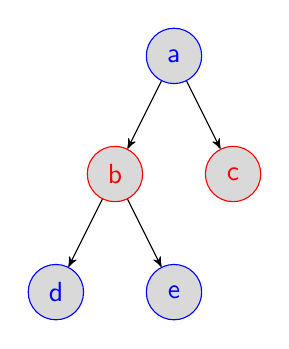
\begin{tikzpicture}
    \node[blue, vertex]
    {a}
        child {
            node[red, vertex] {b}
            child { node[blue, vertex] {d} }
            child { node[blue, vertex] {e} }
        } child {
            node[red, vertex] {c}
        }
    ;
  \end{tikzpicture}
  \begin{tabular}{|l|l|}
  \textb{a} & \textg{a} \\
  \textr{b} & \textr{b} \\
  \textr{c} & \textr{c} \\
  \textb{d} & \textb{d} \\
  \textb{e} & \textb{e} \\
  \hline
  \end{tabular}
\vfill\columnbreak
  (b) \\
  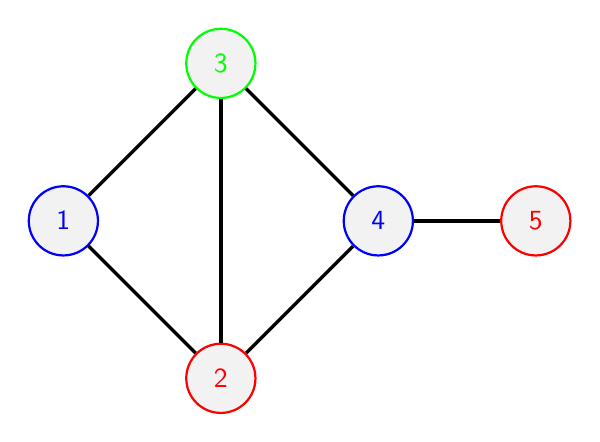
\begin{tikzpicture}[node distance=2cm]
    \node[blue,  state] (1) {1};
    \node[red,   state, below of=1, right of=1] (2) {2};
    \node[green, state, above of=1, right of=1] (3) {3};
    \node[blue,  state, above of=2, right of=2] (4) {4};
    \node[red,   state, right of=4] (5) {5};
    \draw[very thick]
      (1) edge[line] (2)
      (1) edge[line] (3)
      (2) edge[line] (3)
      (2) edge[line] (4)
      (3) edge[line] (4)
      (4) edge[line] (5);
  \end{tikzpicture}
  \begin{tabular}{|l|}
  \textb{1} \\
  \textr{2} \\
  \textg{3} \\
  \textb{4} \\
  \textr{5} \\
  \hline
  \end{tabular}
\end{multicols}
\vspace{-1em}
\begin{description}
  \item [\cmark] (b) is 3-colorable.
  \item [\xmark] (b) is 2-colorable.
  \item [\cmark] (a) is 2-colorable.
  \item [\xmark] Both (a) and (b) are not 2-colorable.
  \item [\cmark] (a) is 3-colorable.
\end{description}

\end{document}